\maketitle

\section{Problema}

Realizar un algoritmo en MatLab que demuestre que la informacion mutua de una concatenacion de enlaces de canales binarios es menor que para un solo enlace.

\begin{figure}[H]
    \centering
    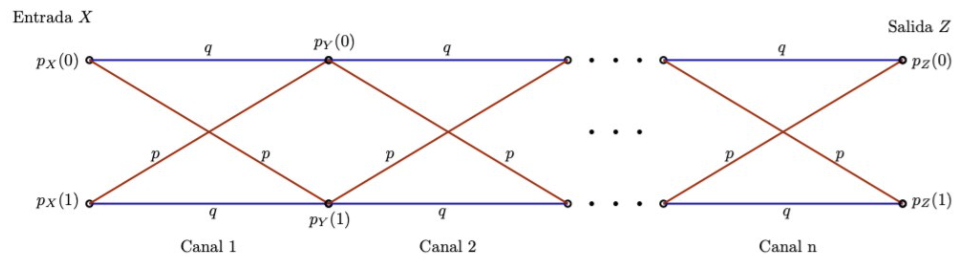
\includegraphics[width=1\textwidth]{taller1/imagenes/canal binario.PNG}
    \caption{\label{fig1}Enlace de comunicaciones}
\end{figure}

\subsection{Solucion}

Para obtener la informacion mutua, se aplica la siguiente ecuacion:

\begin{equation}
    I_{(x;y)}=H_{(x)}-H_{(x|y)}
\end{equation}

Donde:

\begin{equation}
    H_{(x)}=p_{x}\cdot log_{2}(\frac{1}{p_x})
\end{equation}

La incertidumbre promedio viene dada por:

\begin{equation}
    H_{(x|y)}=\sum_{x}\sum_{y}p_{xy(x,y)}\cdot log_{2}(\frac{1}{p_{x|y(x|y)}})
\end{equation}

Para la simulacion de $N$ canales del canal binario, se implementa el siguiente codigo en MatLab.

\begin{figure}[H]
    \centering
    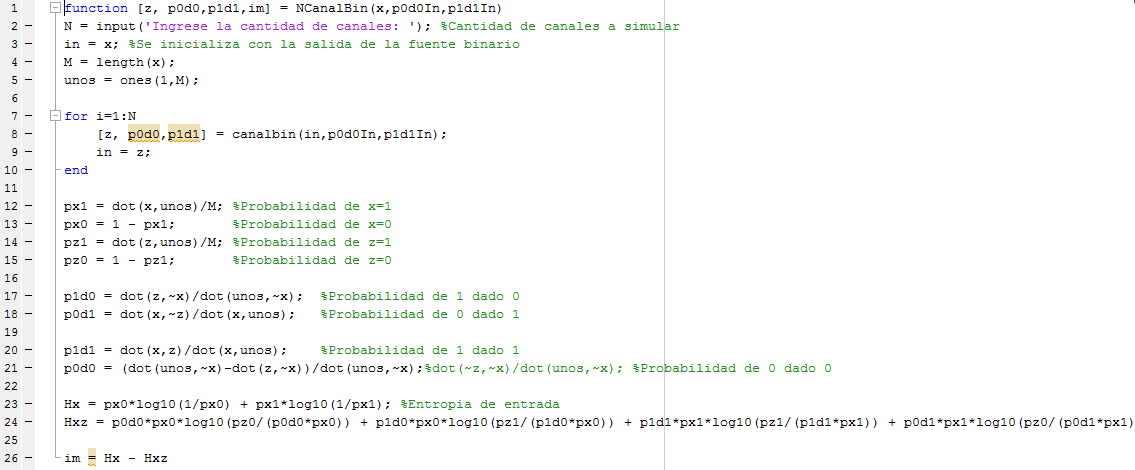
\includegraphics[width=1\textwidth]{taller1/imagenes/codigo canal binario.PNG}
    \caption{\label{fig1}Codigo en Matlab}
\end{figure}

Para este caso, la ecuacion 3 puede ser expresada de la forma:

\begin{equation*}
    H_{(x|y)} = p_{y|x(0|0)}\cdot p_{x(0)}\cdot log_{10}\left(\frac{p_{y(0)}}{p_{y|x(0|0)\cdot p_{x(0)}}}\right)
    +
    p_{y|x(1|0)}\cdot p_{x(0)}\cdot log_{10}\left(\frac{p_{y(1)}}{p_{y|x(1|0)\cdot p_{x(0)}}}\right)+\cdot \cdot \cdot
\end{equation*}

\begin{equation*}
    \cdot \cdot \cdot
    +
    p_{y|x(1|1)}\cdot p_{x(1)}\cdot log_{10}\left(\frac{p_{y(0)}}{p_{y|x(0|1)\cdot p_{x(1)}}}\right)
    +
    p_{y|x(0|1)}\cdot p_{x(1)}\cdot log_{10}\left(\frac{p_{y(0)}}{p_{y|x(0|1)\cdot p_{x(1)}}}\right)
\end{equation*}

Datos que fueron obtenidos en la simulacion, con lo cual se puede determinar la informacion mutua de los $N$ canales.

\subsection{Simulacion}

Se tomaran ciertos casos para comprobar la veracidad del enunciado.
\\
\\
Para $P_{y|x(0|0)} = 0.9$, $P_{y|x(1|1)} = 0.7$ con 1 canal. Simulando varias veces se obtiene un promedio de:

\begin{equation*}
    I_{(x,y)}\approx 0.09352
\end{equation*}

Incrementando los canales a 5:

\begin{equation*}
    I_{(x,y)}\approx 0.00566
\end{equation*}

Ahora con 10 canales:

\begin{equation*}
    I_{(x,y)}\approx 1.1642\cdot 10^{-4}
\end{equation*}

Ahora se obtienen unos valores de las probabilidades de las lineas del canal mas ideales de $P_{y|x(0|0)} = 0.99$, $P_{y|x(1|1)} = 0.99$:

\begin{equation*}
    I_{(x,y)}\approx 0.16826
\end{equation*}

Incrementando los canales a 5:

\begin{equation*}
    I_{(x,y)}\approx 0.0268
\end{equation*}

Ahora con 10 canales:

\begin{equation*}
    I_{(x,y)}\approx 0.00364
\end{equation*}

Se puede destacar una disminucion de $I_{(x,y)}$ a medida que se aumentan los canales, y un aumento a medida que las probabilidades del canal tienden a $1$.
